In this section, we first outline the algorithmic structure of a 
single time step of LESGO. Then, we analyze the scaling limits of 
the CPU implementation that motivate our GPU acceleration strategy.

\subsection{Structure of a Time Step}

\label{sec:step}
\begin{algorithm}[h]
\caption{The main time loop of LESGO.}
\label{alg:step}
\begin{algorithmic}[1]
\STATE \texttt{Initialize()}
\FOR{$n = 1, N$}
\STATE \texttt{ComputeDt()}
\STATE \textcolor{stgderiv}{Derivatives()}\algptr{stgderiv}{sec:method-taxonomy}
\STATE \textcolor{stgderiv}{WallStress()}
\STATE \textcolor{stgsgs}{SGS()}
\STATE \hspace{1.3em}\textbf{if} $n \bmod c = 0$ \textbf{then}
\STATE \hspace{2.6em}\textcolor{stgsgs}{UpdateLASDCoefficient()}\algptr{stgsgs}{sec:opt-lasd}
\STATE \hspace{1.3em}\textcolor{stgsgs}{SGSStress()}
\STATE \hspace{1.3em}\textcolor{stgsgs}{StressDivergence()}
\STATE \textcolor{stgconv}{Convection()}
\STATE \textcolor{stgturb}{Turbines()}
\STATE \hspace{1.3em}\textcolor{stgturb}{SampleBladeVelocities()}\algptr{stgturb}{sec:opt-atm}
\STATE \hspace{1.3em}\textcolor{stgturb}{ComputeBladeForces()}\algptr{stgturb}{sec:opt-overlap}
\STATE \hspace{1.3em}\textcolor{stgturb}{SpreadBladeForces()}\algptr{stgturb}{sec:opt-atm}
\STATE \textcolor{stgpress}{AdvanceAB2()}
\STATE \textcolor{stgpress}{Pressure()}
\STATE \hspace{1.3em}\textcolor{stgpress}{PoissonFFT()}
\STATE \hspace{1.3em}\textcolor{stgpress}{PoissonTridiag()}\algptr{stgpress}{sec:opt-tridag}
\STATE \hspace{1.3em}\textcolor{stgpress}{PoissonInvFFT()}
\STATE \textcolor{stgproj}{ProjectVelocity()}
\ENDFOR
\STATE Finalize()
\end{algorithmic}
\end{algorithm}

LESGO follows a conventional time-marching structure. The solver
state comprises the three filtered velocity components of Eq.~\ref{eq:les},
held on the slab-decomposed grid (Section~\ref{sec:bg-impl}). Each
pass of the main time loop in Algorithm~\ref{alg:step} executes three 
primary phases: (1)~assembling the right-hand-side (RHS) convective, 
turbulent, and boundary force terms (lines 3--15), (2)~advancing the 
velocity to an intermediate state via second-order
Adams--Bashforth integration (line 16), and (3)~enforcing incompressibility 
through a Poisson pressure solve and velocity projection step (lines 17--21). 
\texttt{Initialize()} allocates grid arrays, creates FFT plans, and sets up 
turbine geometry at startup, while \texttt{Finalize()} outputs final diagnostics 
and checkpoints. Inside the loop, \texttt{ComputeDt()} dynamically evaluates 
the time step according to the Courant--Friedrichs--Lewy (CFL) stability 
condition, requiring a global \texttt{MPI\_Allreduce} collective across all ranks.
Below, we describe the execution flow of a single time step in detail.

\stagelead{stgderiv}{Derivatives} (lines 4--5). Evaluating the RHS
terms of Eq.~\ref{eq:les} requires velocity gradients, since the SGS
stress depends on the strain-rate tensor and the rotational convective
term on vorticity. Horizontal derivatives are computed spectrally via
2D forward and inverse FFTs on each $x$-$y$ plane, whereas vertical
derivatives use second-order centered differences that read one ghost
plane exchanged with neighbor ranks. This operation forms a uniform,
memory-streaming sweep across the 3D domain. \texttt{WallStress()}
then applies the logarithmic law-of-the-wall model
(Section~\ref{sec:bg-numerics}) to compute surface shear stress on
the boundary ranks.

\stagelead{stgsgs}{SGS} (lines 6--10). Subgrid-scale closure models the 
unresolved turbulent fluxes. Every $c$-th step ($c=5$ in production runs), 
\texttt{UpdateLASDCoefficient()} updates the dynamic Lagrangian scale-dependent (LASD) 
model coefficient $C_s^2$ (Section~\ref{sec:bg-physics}) by applying two 
spectral test filters and advecting dynamic model accumulators along fluid particle 
trajectories, making it the most computationally irregular and memory-bound routine 
in the solver (Section~\ref{sec:opt-lasd}). On every step, \texttt{SGSStress()} 
recalculates the eddy viscosity $\nu_t = C_s^2 \Delta^2 |S|$ using the current 
strain rate and computes the subgrid stress tensor, after which 
\texttt{StressDivergence()} calculates its spatial divergence.

\stagelead{stgconv}{Convection} (line 11). To eliminate aliasing errors 
arising from non-linear convective terms in rotational form, LESGO employs 
the standard $3/2$-rule dealiasing scheme. Each velocity and vorticity 
component undergoes forward and inverse 2D horizontal FFTs on an
expanded ($1.5\times$ padded) grid. Convection represents the most 
FFT-intensive phase of the time step.

\stagelead{stgturb}{Turbines} (lines 12--15). The actuator-line model 
(ALM) represents wind turbine blades as localized aerodynamic force 
sources in Eq.~\ref{eq:les}. \texttt{SampleBladeVelocities()}
samples flow velocities at discrete blade actuator points via 
trilinear 3D spatial interpolation.
\texttt{ComputeBladeForces()} calculates angle of attack, 
relative velocity, and lift/drag forces using lookup tables of empirical 
airfoil polar data. Finally, \texttt{SpreadBladeForces()} projects
these forces back onto surrounding fluid grid points using 3D Gaussian
spatial regularization.

\stagelead{stgpress}{Pressure} (lines 16--20). The intermediate velocity 
field computed by \texttt{AdvanceAB2()} is generally not divergence-free, so 
its divergence acts as the source term for a 3D Poisson equation for
modified pressure. \texttt{PoissonFFT()} transforms the RHS into
horizontal wave space, decoupling horizontal modes into independent
1D vertical tridiagonal linear systems along $z$. \texttt{PoissonTridiag()}
solves these systems across the MPI rank stack (Section~\ref{sec:opt-tridag}),
and \texttt{PoissonInvFFT()} returns the pressure and its horizontal
gradients to physical space, with the vertical gradient evaluated by
finite differencing. Pressure is the only solver stage requiring
fine-grained, globally coupled communication across all vertical ranks.

\stagelead{stgproj}{Projection} (line 21). \texttt{ProjectVelocity()} 
subtracts the pressure gradient from the intermediate velocity to project 
the flow onto solenoidal (divergence-free) space. Finally, point-to-point 
halo exchanges refresh the single-plane ghost layers to prepare velocity 
fields for the subsequent time step's derivative calculations.

\subsection{MPI Slab Decomposition and Scaling Ceiling}
\label{sec:bg-impl}

LESGO is implemented in Fortran~90 and parallelized with MPI using a 1D slab 
decomposition along the vertical ($z$) axis. Each MPI rank owns a contiguous 
block of horizontal $z$-planes spanning the full horizontal domain ($x$-$y$). 
This topology allows 2D horizontal FFTs to execute entirely rank-locally,
completely avoiding expensive 2D domain transposes (\texttt{MPI\_Alltoallv})
required by 2D pencil decompositions~\cite{romero2022}. Primary physical 
fields, including velocity components, modified pressure, and subgrid 
turbulence scalars, are stored as 3D Fortran arrays.

Inter-rank communication in this slab topology follows three main patterns.
First, vertical finite-difference stencils require nearest-neighbor halo 
exchanges of single horizontal planes between adjacent ranks. Second, 
the pressure Poisson solve induces global coupling across all ranks, 
as each vertical tridiagonal system spans the entire domain height after 
horizontal spectral transformation (Section~\ref{sec:opt-tridag}).
Third, small collective reductions execute CFL time-step control, runtime 
diagnostic logging, and per-turbine force aggregation. By avoiding 2D 
domain transposes, this 1D slab decomposition keeps computationally 
intensive horizontal FFTs rank-local at the expense of a globally coupled 
vertical solve.

\begin{figure}[h]
    \centering
    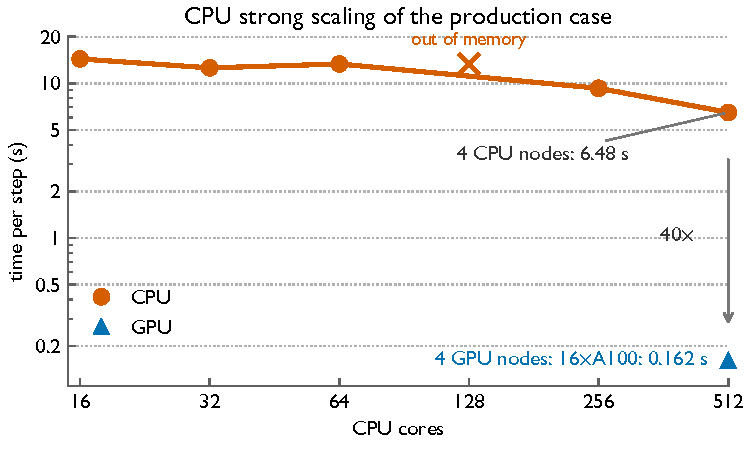
\includegraphics[width=\linewidth]{figs/fig_ceiling.pdf}
    \caption{CPU strong scaling of LESGO on the production wind-farm case of Section~\ref{sec:setup}.}
    \label{fig:ceiling}
\end{figure}
    

On CPU architectures, this design encounters severe scaling limits.
Figure~\ref{fig:ceiling} evaluates the strong scaling of the production
wind-farm case, which simulates 60 turbines on a 472M-cell grid
($3072 \times 384 \times 400$), on Perlmutter CPU nodes with
two 64-core AMD EPYC 7763 (Milan) CPUs each.
As shown in Figure~\ref{fig:ceiling}, the bandwidth-bound solver
saturates a node near 40 of its 128 cores (9.68\,s per step), and
packing 100 ranks onto the same node is counterproductive (11.4\,s).
Scaling out helps only weakly. Two nodes at 200 ranks reach 7.29\,s,
and four nodes at 400 ranks, where the 1D slab decomposition reaches
its structural limit of one vertical plane per rank, plateau at
5.11\,s per step.
At this scaling ceiling, accumulating converged turbulence statistics
requires running hundreds of thousands of time steps. As a result, a single
production simulation takes several hours to days to complete, making
large-scale wind-farm studies computationally impractical. This significant
performance gap motivated our development of the GPU port.
